\section{INTERPLIN1 Linear 1-D Interpolation}

\subsection{Usage}

Given a set of monotonically increasing \verb|x| coordinates and a 
corresponding set of \verb|y| values, performs simple linear 
interpolation to a new set of \verb|x| coordinates. The general syntax
for its usage is
\begin{verbatim}
   yi = interplin1(x1,y1,xi)
\end{verbatim}
where \verb|x1| and \verb|y1| are vectors of the same length, and the entries
in \verb|x1| are monotoniccally increasing.  The output vector \verb|yi| is
the same size as the input vector \verb|xi|.  For each element of \verb|xi|,
the values in \verb|y1| are linearly interpolated.  For values in \verb|xi| 
that are outside the range of \verb|x1| the default value returned is
\verb|nan|.  To change this behavior, you can specify the extrapolation
flag:
\begin{verbatim}
   yi = interplin1(x1,y1,xi,extrapflag)
\end{verbatim}
Valid options for \verb|extrapflag| are:
\begin{itemize}
\item  \verb|'nan'| - extrapolated values are tagged with \verb|nan|s

\item  \verb|'zero'| - extrapolated values are set to zero

\item  \verb|'endpoint'| - extrapolated values are set to the endpoint values 

\item  \verb|'extrap'| - linear extrapolation is performed

\end{itemize}
The \verb|x1| and \verb|xi| vectors must be real, although complex types
are allowed for \verb|y1|.
\subsection{Example}

Here is an example of simple linear interpolation with the different
extrapolation modes.  We start with a fairly coarse sampling of a 
cosine.
@>
which is shown here


\centerline{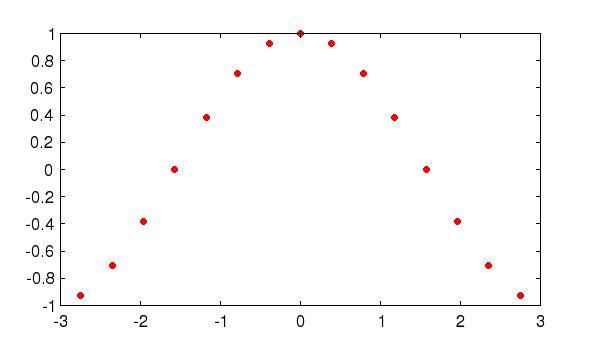
\includegraphics[width=8cm]{interplin1_1}}

Next, we generate a finer sampling over a slightly broader range
(in this case \verb|[-pi,pi]|).  First, we demonstrate the \verb|'nan'| 
extrapolation method
@>
which is shown here


\centerline{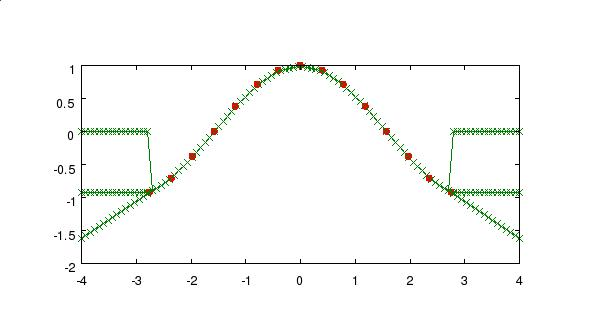
\includegraphics[width=8cm]{interplin1_2}}

